% !TEX root=/home/tavant/these/manuscript/src/manuscript.tex

% \FloatBarrier

\section{Comparison of the sheath model with PIC simulations} \label{subsec-picandmodel}

% \begin{figure}[hbtp]
%   \centering
%   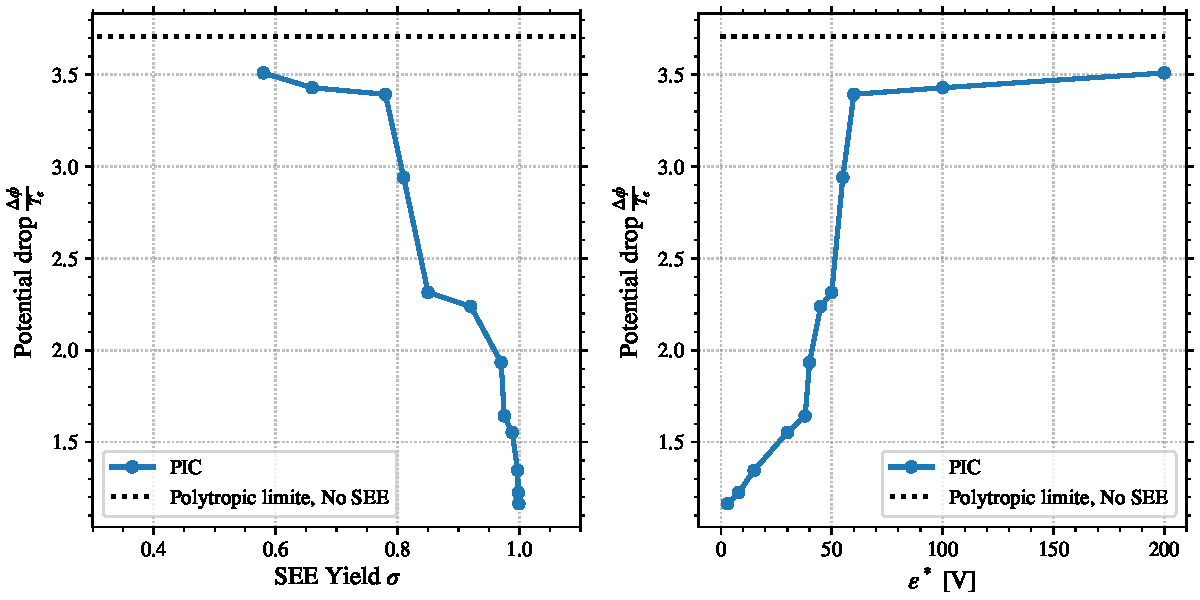
\includegraphics[width=\textwidth]{dphi_polytropic_noSEE}
%   \caption{PIC simulation results (with SEE) compared to the polytropic limit without SEE.}
%   \label{fig-polytropic_pic_noSEE}
% \end{figure}
% 
% \begin{figure}[hbtp]
%   \centering
%   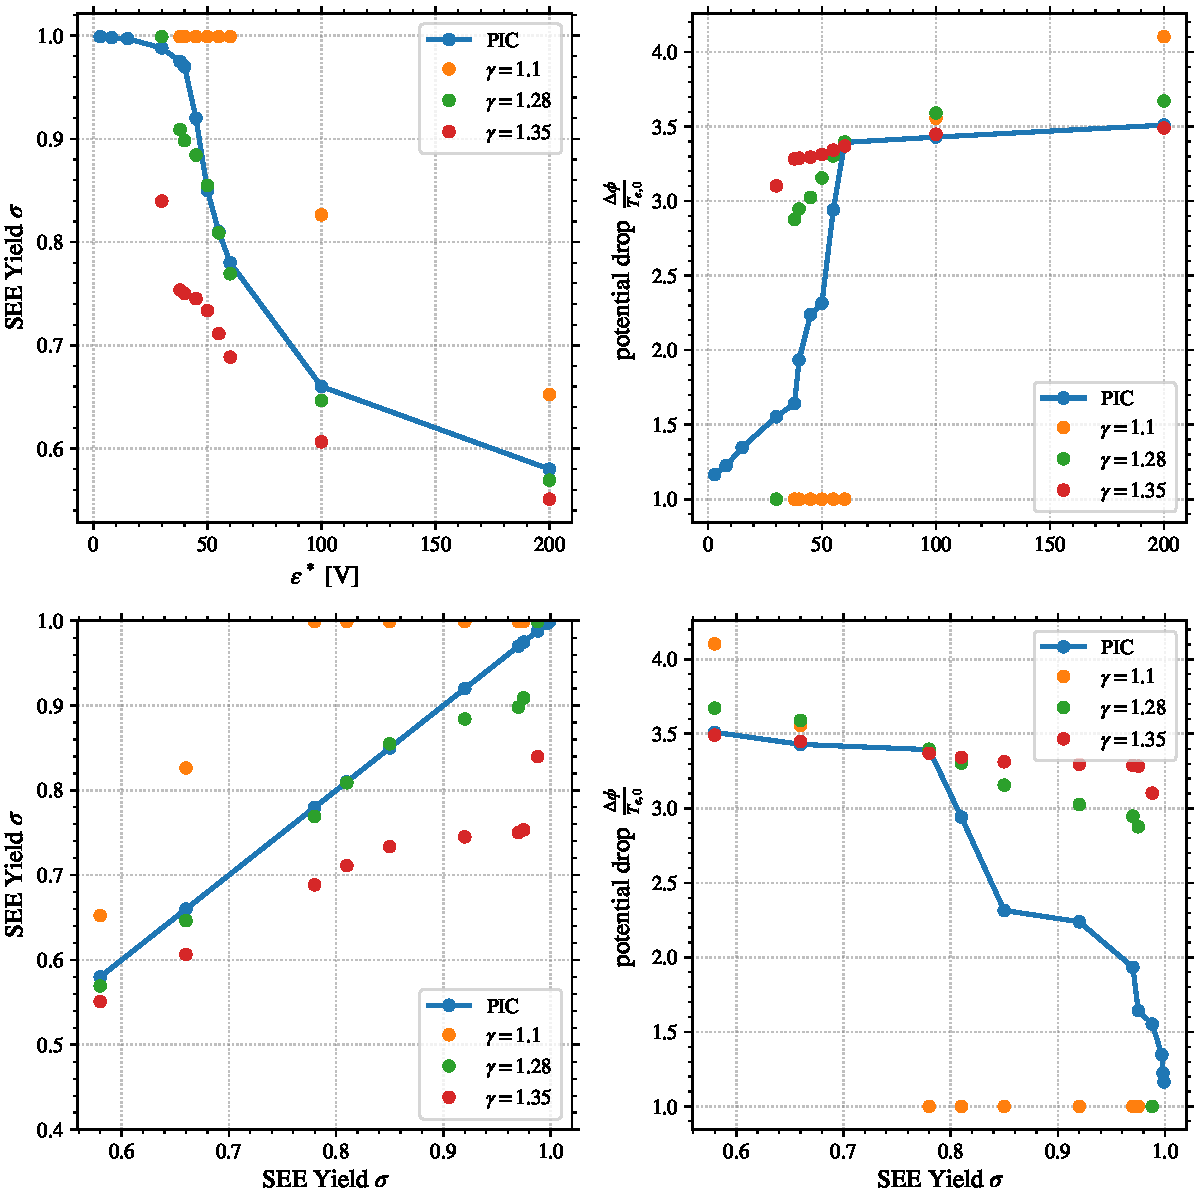
\includegraphics[width=\textwidth]{Summary_polytropic_SEE.pdf}
%   \caption{Comparison of the PIC simulation results with the polytropic model with SEE.}
%   \label{fig-polytropic_see_summary}
% \end{figure}

We compare in this section the characteristics of the plasma wall interaction observed in the \ac{PIC} simulations with the fluid model developed in \cref{sec-fluid_poly_see}.
The variables of interest are the averaged electron emission rate $\rate$ and the plasma potential drop to the wall.
The only input of the model is the electron mean temperature in the bulk $\Teb$ as well as the polytropic index $\gamma$.
As seen in \cref{sec-PIC_poly}, the polytropic index of the electron population is measured in the \ac{PIC} simulation to $\gamma=1.35$.
However, the electrons going toward the wall present a different index, measured from the bulk \ac{EVDF} to $\gamma=1.28$.
These two values will be compared.

Using the mean electron temperature measured in the simulation, we first compute the plasma potential drop $\dphi$ by solving \cref{eq-costseepoly} with $\gamma=1.35$.
As showed in \cref{fig-rso_crit_see}, up to three solutions are possible.
The emission rate $\rate$ is then computed using \cref{eq-seemaxw_Tew}, using the two values for $\gamma$.
As discussed previously, the rate is limited to $\ratecr=0.982$ to take into account the \ac{SCL} regime.

The results are shown in \Cref{fig-Poly_model_vs_pic}.
The plasma potential drop computed is increased by $\Teb/2$ corresponding to the pre-sheath drop to better match the plasma potential measured in the simulations.
\improvement{The Bhom criterion is slightly modified with the polytropic model, so it should not exactly be $\Teb/2$. however, it matches to well here that I do not really want to change !}

\begin{figure}[hbtp]
  \centering
  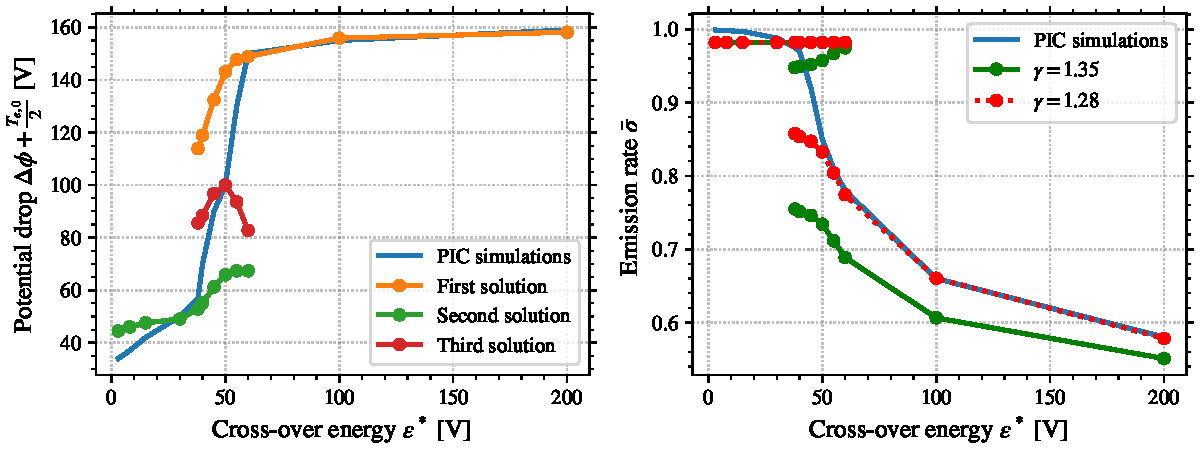
\includegraphics[width=\textwidth]{Poly_model_vs_pic}
  \caption{Comparison of the PIC simulations and the sheath model for the plasma potential drop from the center to the wall and the electron emission yield. }
  \label{fig-Poly_model_vs_pic}
\end{figure}

Concerning $\dphi$, we can see that the sheath model combining the polytropic state law and the electron emission is in good agreement with the \ac{PIC} simulations.
We can see that the region where the three solutions coexist corresponds well with the regime {\bf II}.

For the emission rate $\rate$, we observe that the value $\gamma=1.35$ under estimates $\rate$ compared to the values of the \ac{PIC} simulations.
On the other hand, $\gamma=1.28$ is in very good agreement.

Interestingly, at the saturation the mean electron emission rate in the \ac{PIC} simulation is greater than the critical value $\ratecr$.
\inlinenote{ As $\rate$ is better with $\gamma=1.28$, we should use both values in \cref{eq-costseepoly}. However, this increases the complexity the equations and the model, and add 1 more free parameters (they would be 2 values for $\gamma$ now). I can say that only in the discussion maybe ? }
